\documentclass[10pt]{amsart}
\usepackage[a4paper,margin=22mm]{geometry}
\usepackage[no-math]{fontspec}
\setmainfont{Latin Modern Roman}[SmallCapsFont={lmromancaps10-regular.otf}]
\usepackage{amsmath,amssymb,amsthm,mathtools,hyperref,etoolbox,tikz,ytableau}
% The original shuffle/pshu definitions are retained, but no shuffle symbol is used in this bounded unit.
\hypersetup{hidelinks}
\emergencystretch=3em
\newtheorem{theo}{Theorem}[section]
\newtheorem{lemma}[theo]{Lemma}
\newtheorem{lemm}[theo]{Lemma}
\newtheorem{prop}[theo]{Proposition}
\newtheorem{coro}[theo]{Corollary}
\newenvironment{enonce*}[2][]{\par\smallskip\noindent\textit{#2.}\ }{\par\smallskip}
\DeclareMathOperator{\std}{std}
\DeclareMathOperator{\SSYT}{SSYT}
\DeclareMathOperator{\RS}{RS}
\DeclareMathOperator{\MaR}{MR}
\DeclareMathOperator{\Pk}{Pk}


\newcommand{\shu}{\shuffle}
\newcommand{\pshu}{\hspace{2pt}\ol{\shu}\hspace{2pt}}
\newcommand{\ofS}{\ol{\fS}}
\newcommand{\lab}{\ol{\la}}
\newcommand{\cHb}{\ol{\cH}}


\newcommand{\comp}{\models}
\newcommand{\ol}{\overline}
\newcommand{\emp}{\emptyset}
\newcommand{\sbs}{\subset}
\newcommand{\sbe}{\subseteq}
\newcommand{\ptn}{\vdash}


\newcommand{\ree}[1]{\eqref{#1}}
\newcommand{\ra}{\rightarrow}

\newcommand{\al}{\alpha}
\newcommand{\be}{\beta}
\newcommand{\de}{\delta}
\newcommand{\io}{\iota}
\newcommand{\ka}{\kappa}
\newcommand{\la}{\lambda}
\newcommand{\si}{\sigma}

\newcommand{\Th}{\Theta}

\newcommand{\bx}{\mathbf{x}}

\newcommand{\bbQ}{{\mathbb Q}}

\newcommand{\cA}{{\mathcal A}}
\newcommand{\cH}{{\mathcal H}}
\newcommand{\cP}{{\mathcal P}}
\newcommand{\cS}{{\mathcal S}}
\newcommand{\cT}{{\mathcal T}}
\newcommand{\cZ}{{\mathcal Z}}

\newcommand{\fS}{{\mathfrak S}}

\newcommand{\Hb}{\ol{H}}

\DeclareMathOperator{\des}{des}
\DeclareMathOperator{\Des}{Des}
\DeclareMathOperator{\sh}{sh}
\DeclareMathOperator{\Sym}{{Sym}}
\DeclareMathOperator{\QSym}{{QSym}}
\DeclareMathOperator{\SYT}{SYT}

\newcommand{\dil}{\displaystyle}

\newcommand\llbracket{[\![}
\newcommand\rrbracket{]\!]}



\title[Pattern-Knuth-closed insertion classes]{Pattern-Knuth-closed insertion classes are exactly superstandard hooks}
\author[Z. Hamaker, B. Pawlowski, and B. E. Sagan]{Zachary Hamaker, Brendan Pawlowski, and Bruce E. Sagan}
\date{Algebraic Combinatorics 3(2)(2020),365–388; DOI10.5802/alco.96}
\AtBeginDocument{\let\originalRef\ref\renewcommand{\ref}[1]{\ifstrequal{#1}{S3}{\href{https://doi.org/10.5802/alco.96}{1 (source)}}{\originalRef{#1}}}}
\begin{document}
\maketitle
\section*{Original notation and Robinson--Schensted prerequisites}
Let $\fS_n$ be the symmetric group of all permutations of $[n]=\{1,\dots,n\}$. We view the permutations in $\fS_n$ as sequences $\pi=\pi_1\dots\pi_n$. Given any sequence $\si$ of $k$ distinct integers, its \emph{standardization} is the permutation $\std\si\in\fS_k$ obtained by replacing the smallest element of $\si$ by $1$, the next smallest by $2$, and so forth. We say that permutation $\si$ \emph{contains permutation $\pi$ as a pattern} if there is a subsequence $\si'$ of (not necessarily consecutive) elements of $\si$ such that $\std\si'=\pi$. For example, $\si=5132746$ contains $\pi=231$ because of the subsequence $\si'=574$.
Permutation $\si$ \emph{avoids} $\pi$ if it does not contain $\pi$ as a pattern. Given a set of permutations $\Pi$ we let 
\[
\fS_n(\Pi) =\{\si\in\fS_n \mid \text{$\si$ avoids every $\pi\in\Pi$}\}.
\]
For more information about permutation patterns, see the book of B\'ona~\cite{bon:cp}. Our object is to make a connection between the theory of patterns and the theory of quasisymmetric functions. First we will review some material concerning symmetric functions. Details about symmetric functions and related combinatorics such as the Robinson--Schensted map can be found in the texts of Macdonald~\cite{mac:sfh}, Sagan~\cite{sag:sym}, or Stanley~\cite{sta:ec2}.

Let $\bx=\{x_1,x_2,\dots\}$ be a countably infinite set of commuting variables and consider the algebra of formal power series over the rationals $\bbQ\llbracket \bx\rrbracket$. Consider a monomial $m=x_{i_1}^{n_1}\dots x_{i_k}^{n_k}$. The \emph{degree} of $m$ is $\sum_i n_i$, and the \emph{degree} of any $f\in\bbQ\llbracket \bx\rrbracket$ is the maximum degree of a monomial in $f$ if the maximum exists or infinity otherwise. We say that $f$ is \emph{symmetric} if it is of bounded degree and invariant under permutation of variables. 
We will be particularly interested in the important Schur basis for $\Sym_n$. Recall that a partition $\la=(\la_1,\dots,\la_k)$ has an associated \emph{Young diagram} consisting of $k$ left-justified rows of boxes with $\la_i$ boxes in row $i$. We will write our diagrams in English notation with the first row on top and often make no distinction between a partition and its diagram. Given $\la\ptn n$ then a \emph{standard Young tableau (SYT)}, $P$, of shape $\la$ is obtained by filling the boxes bijectively with the elements of $[n]$ so that rows and columns increase. In a \emph{semistandard Young tableau (SSYT)}, $T$, of shape $\la$ the entries are positive integers distributed so that rows weakly increase and columns strictly increase. 
We write $\SYT(\la)$ or $\SSYT(\la)$ for the set of standard or semistandard Young tableaux of shape $\la$, respectively. 
We also write $\sh P=\la$ or $\sh T=\la$ to indicate that $P$ or $T$ have shape $\la$.
To combine permutation patterns and quasisymmetric functions, recall that the \emph{descent set of a permutation}
$\pi=\pi_1\dots\pi_n$ is
\[
\Des\pi=\{i \mid \pi_i>\pi_{i+1}\}\sbe[n-1].
\]
\setcounter{section}{2}\setcounter{theo}{1}

In order to deal with reversals, we will need some background about the Robinson--Schensted map~\cite{rob:rsg,sch:lid}. This is a bijection
\[
\RS:\fS_n\ra\bigcup_{\la\ptn n} \SYT(\la)\times\SYT(\la).
\]
If $\RS(\pi)=(P,Q)$ then we will write $P=P(\pi)$ and $Q=Q(\pi)$ and call $P$ and $Q$ the \emph{$P$-tableau} and \emph{$Q$-tableau} of $\pi$, respectively.
If $\pi=\pi_1\dots\pi_n$ then $P$ is constructed using an operation called \emph{insertion} that sequentially inserts $\pi_1,\dots,\pi_n$ to form $P$. After the $k$th insertion, a $k$ is \emph{placed} in $Q$ so that one maintains $\sh P=\sh Q$ at all times. Although we are using $Q$ in both the notation $Q(\pi)$ and $Q_n(\Pi)$ the two different concepts should be distinguishable by context and the fact that the latter has a subscript while the former does not. 

\looseness-1
We put an equivalence relation on $\fS_n$ by declaring that $\pi$ and $\si$ are \emph{Knuth equivalent}, written $\pi\sim\si$, if $P(\pi)=P(\si)$. Given an SYT $P$, the corresponding \emph{Knuth class} is
\[
K(P) = \{\pi \mid P(\pi)=P\}.
\]
\looseness-1
Given a partition $\la$ it will also be convenient to define an associated \emph{Knuth aggregate}~by
\[
K(\la) = \{\pi \mid \sh P(\pi) = \la\} =\bigcup_{\sh(P)=\la} K(P).
\]
We will need the following properties of the map $\RS$. For proofs of these results, see~\cite{sta:ec2}.
\begin{theo}
\label{RS}
Suppose $\RS(\pi)=(P,Q)$.
\begin{enumerate}
\item\label{theo2.2_a} %[(a)] 
$\Des\pi=\Des Q$.
\item\label{theo2.2_b} %[(b)] 
If $\sh P=\la$ then $\la_1$ is the length of a longest increasing subsequence of $\pi$.
\item\label{theo2.2_c} %[(c)] 
$P(\pi^r) = (P(\pi))^t$.
\item\label{theo2.2_d} %[(d)] 
$\RS(\pi^{-1}) = (Q,P)$. %\hqed
\end{enumerate}
\end{theo}
\setcounter{section}{4}
\section{Knuth classes}
\label{kc}

The final entries from Table~\ref{S3} that need to be explained are $\{132, 312\}$ and $\{213,231\}$. The reader will recognize these as Knuth classes $K(P)$ for $P$ equal to
\begin{equation}
\label{12:3}
\begin{ytableau} 1&2\\ 3 \end{ytableau}
\end{equation}
and
\begin{equation}
\label{13:2}
\begin{ytableau} 1&3\\ 2 \end{ytableau}\ ,
\end{equation}
respectively. The main result of this section will be a characterization of the $P$ for which $\fS_n(K(P))$ is a union of Knuth classes for all $n$. For such $P$ it is clear that $Q_n(K(P))$ will be Schur nonnegative. We will first deal with the special case when $P$ is one of the two tableaux above.
\setcounter{theo}{1}
We now consider general Knuth classes $K(P)$. We first need to recall some general facts about these sets. Suppose we have positive integers $a<b<c$ and a permutation $\si$ having a factor (subsequence of consecutive elements) $acb$ or $cab$. Then we can perform a \emph{Knuth move} on $\si$ by exchanging one factor for the other. Alternatively, a Knuth move can exchange factors of the form $bac$ and $bca$. Two permutations are \emph{Knuth equivalent} if one can be transformed into the other by a sequence of Knuth moves. For a proof of the next result, see~\cite{sag:sym}.
\begin{theo}
\label{Kequiv}
If $P(\si)=P$ then $K(P)$ is the set of permutations Knuth equivalent to $\si$. %\hqed
\end{theo}

Call $\Pi$ \emph{pattern-Knuth closed} if $\fS_n(\Pi)$ is a union of Knuth classes for all $n$. Equivalently, the complement $\ofS_n(\Pi)$ is a union of Knuth classes for all $n$. The following lemma is easy to prove directly from the definitions so its demonstration is omitted.
\begin{lemma}
\label{pkc:rc}
If $\Pi$ is pattern-Knuth closed then so are $\Pi^c, \Pi^r,$ and $\Pi^{rc}$. %\hqed
\end{lemma}

There is a sense in which this property is stable.
\begin{lemma}
\label{pkc:M}
The set $\Pi$ is pattern-Knuth closed if and only if $\fS_n(\Pi)$ is a union of Knuth classes for $n\le M+1$ where $M$ is the maximum length of a permutation in $\Pi$.
\end{lemma}
\begin{proof}
The forward direction is obvious so we will prove the converse. It will be more convenient to show that $\ofS_n(\Pi)$ is a union of Knuth classes for $n>M+1$. Suppose $\si\in\ofS_n(\Pi)$ contains a copy $\ka$ of some $\pi\in\Pi$. By Theorem~\ref{Kequiv}, it suffices to show that the result $\si'$ of performing a Knuth move on $\si$ will still be in $\ofS_n(\Pi)$. We will do this for a factor $acb$ where $a<b<c$ as the other possible Knuth moves can be handled similarly. There are three cases.

If $\ka$ does not contain both $a,c$ then $\ka$ is still a subsequence of $\si'$ and we are done. If $\ka$ contains all three elements, then $\si'$ contains $\ka'$, which is formed by replacing $acb$ by $cab$ in $\ka$. Since our hypothesis implies that $\Pi$ is a union of Knuth classes, $\ka'$ is a copy of an element of $\Pi$ and we are again finished. The final case is when $a,c$ are in $\ka$ but $b$ is not. Let $\pi'$ be the standardization of the subsequence of $\si$ containing $\ka$ and $b$. Then $\pi'\in\ofS_n(\Pi)$ for some $n\le M+1$. It follows from the hypothesis in this direction that the permutation $\pi''$ obtained by switching the elements corresponding to $a,c$ in $\pi'$ still contains an element of $\Pi$. Since $\si'$ contains a copy of $\pi''$ this finishes the proof.
\end{proof}
\setcounter{theo}{6}
We need one more result before we prove the main theorem of this section. For $J\sbe [n-1]$ we let
\[
D_J =\{\pi\in\fS_n \mid \Des\pi= J\}.
\]
Suppose that $\RS(\pi)=(P,Q)$. Then, by Theorem~\ref{RS}~\eqref{theo2.2_a}, we have $\pi\in D_J$ if and only if $\Des Q= J$. As with other operations, we apply the inverse operator to a set of permutations by applying it to each individual permutation. It now follows from what we have just said and Theorem~\ref{RS}~\eqref{theo2.2_d} that $\pi\in D_J^{-1}$ if and only if $\Des P = J$. Then $D_J^{-1}$ is a union of Knuth classes. Also, it follows easily from the definitions that $\Des(\pi^{-1})$ is the set of all $i$ such that $i+1$ appears to the left of $i$ in $\pi$. These two observations are important for the proof of the following result.
\begin{lemma}
\label{DJ-1}
For any $J$, the set $D_J^{-1}$ is pattern-Knuth closed.%\hqed
\end{lemma}
\begin{proof}
The proof is very similar to that of Lemma~\ref{pkc:M}. We only need to take some care with the last case for which we use the same notation as in that demonstration. Suppose first that the elements of $\pi$ corresponding to $a,c$ in $\ka$ are not consecutive in value. From the discussion before the lemma, switching them will result in $\ka'$ whose standardization has the same inverse descent set as $\ka$, namely $J$. Thus $\si'\in\ofS_n(D_J^{-1})$. Now suppose that $a$ and $c$ standardize respectively to $i$ and $i+1$ in $\pi$. It follows that the other elements of $\ka$ are all less than $a$ or greater than $c$. Now let $\ka'$ be $\ka$ with $c$ replaced by $b$. Since $a<b<c$ we have that $\ka'$ also standardizes to $\pi$, and $\ka'$ is a subsequence of $\si'$, finishing this subcase.
\end{proof}

To state our principal result, we need one last set of definitions. The \emph{row superstandard} Young tableau of shape $\la$ is the SYT obtained by filling the first row with $1,2\dots,\la_1$; the next row with $\la_1+1,\la_1+2,\dots,\la_1+\la_2$; and so on. Note that the tableau in~\ree{12:3} is row superstandard. 
A \emph{column superstandard} Young tableau is defined similarly except that one fills the columns from left to right; see~\ree{13:2}. A tableau of either type is just called \emph{superstandard}


\begin{theo}
\label{pkc:main}
The class $K(P)$ is pattern-Knuth closed if and only if $P$ is a superstandard tableau of hook shape.
\end{theo}

We will prove this in a sequence of propositions which deal with the various cases involved. Note that because of Theorem~\ref{RS}~\eqref{theo2.2_c} and Lemma~\ref{pkc:rc} we have $K(P)$ is pattern-Knuth closed if and only if $K(P^t)$ is. Therefore we only need to prove closure, or lack thereof, for one of $P$ or $P^t$. We also assume throughout that the shape of $P$ is $\lambda\ptn n$.


\begin{prop}
\label{p:hook_closed}
If $P$ is superstandard of hook shape then $K(P)$ is pattern-Knuth closed.
\end{prop}
\begin{proof}
Suppose $\la=(n-k, 1^k)$. By the remarks just before this proposition it suffices to prove this when $P$ is column superstandard. It is easy to see that in this case $K(P)=D_J^{-1}$ where $J=[k]$. The result then follows from Lemma~\ref{DJ-1}.
\end{proof}

It will be convenient in our proofs to work with permutations and SYT having elements that are rational numbers, not just integers. To this end, given an integer $a$ we let $a^+= a + 1/2$ and $a^- = a - 1/2$. It will be important when comparing such permutations and tableaux that we always standardize them to have entries $[n]$ for some $n$. 
We will also need the \emph{column reading word} of an SYT $P$, which is the permutation $\rho(P)$ obtained by recording the elements in each column of $P$ read bottom to top and then concatenating the sequences for the columns left to right. It is easy to see that the insertion tableau of $\rho(P)$ is $P$.

\begin{prop}
If $P$ is of hook shape but not superstandard then $K(P)$ is not pattern-Knuth closed.
\end{prop}
\begin{proof}
Our strategy, as suggested by Lemma~\ref{pkc:M}, will be to find an element $\si\in\ofS_{n+1}(K(P))$ to which a Knuth move can be applied creating a permutation $\si'$ having no subsequence $\ka$ with $\std P(\ka)=P$. By transposition if necessary, we can assume that $n$ is in the first column of $P$. Since $P$ is not superstandard, there is some $a>1$ in its first column such that $a+1$ is in the first row of $P$. Let $a$ be the largest such element. Let $b>a+1$ be the next element in $P$'s first column so that we have the following situation
\[
P=
\raisebox{15mm}{\ytableausetup
{boxsize=1.7em}
\begin{ytableau}
1 & \cdots & \scriptstyle a{+}1 & \cdots\\
\vdots\\
a\\
b\\
\vdots\\
n
\end{ytableau}}
\]
with $b+1$ being in the first column if $b<n$.

Let $\si$ be the permutation obtained by placing $a^+$ just before $b \in \rho(P)$ so that
\[
\si = n, \dots, a^+, b, a, \dots
\]
which by construction is an element of $\ofS_{n+1}(K(P))$. Now exchange $a$ and $b$ to obtain 
\[
\si'= n,\dots,a^+,a,b,\dots
\]
Knuth equivalent to $\si$.
Let $\ka$ be any subsequence of $\si'$ with $|\ka|=n$ and suppose $k$ is the element removed to form $\ka$. If $k=b$ then the first column of $P(\ka)$ contains $a^+$, which standardizes to $a+1$ so that $\std P(\ka)\neq P$. If $k\neq b$ then when $b$ is inserted it will enter the tableau in box $(1,2)$ since either $a$ or $a^+$ will be in box $(1,1)$ at that point. When $P(\ka)$ is standardized, $b$ will either stay the same or be replaced by $b+1$. But both those elements need to be in the first column, so at some point $b$ will be bumped out of the first row. But then it will enter the second row in box $(2,2)$ because at least two of $1,a,a^+$ are in $\ka$ so that the element in box $(2,1)$ when $b$ is bumped will be $a$ or smaller. Then there will be a $(2,2)$ entry in $P(\ka)$ forcing its shape not to be a hook, which completes our proof.
\end{proof}

Note that by performing transpositions, it suffices to prove Theorem~\ref{pkc:main} for tableaux $P$ satisfying $P_{2,1}=2$.

\begin{prop}
Let $P$ be a standard tableau of non-hook shape with $P_{2,1}=2$. If there exists an $i$ with $P_{i,1}>P_{i-1,2}$ then $K(P)$ is not pattern-Knuth closed.
\end{prop}
\begin{proof}
We will use the strategy and notation of the proof of the previous proposition. We can write $P$ in the following form
\[
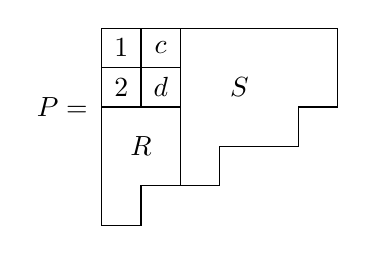
\begin{tikzpicture}[scale=.5]
\node at (-1,-2) {$P=$};
\draw (0,0) to (6,0) to (6,-2) to (5,-2) to (5,-3) to (3,-3) to (3,-4) to (2,-4) to (2,0);
\draw (0,-1) to (2,-1);
\draw (1,0) to (1,-2);
\draw (0,0) to (0,-5) to (1,-5) to (1,-4) to (2,-4) to (2,-2) to (0,-2);
\node at (.5,-.5) {$1$};
\node at (.5,-1.5) {$2$};
\node at (1.5,-.5) {$c$};
\node at (1.5,-1.5) {$d$};
\node at (1,-3) {$R$};
\node at (3.5,-1.5) {$S$};
\end{tikzpicture}.
\]
It is easy to see that the insertion tableau of $\pi= \rho(R), 2, d, 1, c, \rho(S)$ is $P$. We consider
\[
\si = \rho(R), 2, d, 2^+, 1, c, \rho(S),
\]
which is Knuth equivalent to
\[
\si' = \rho(R), d, 2, 2^+, 1, c, \rho(S).
\]
Remove an element $k$ from $\si'$ to form $\ka$. There are two cases.

Suppose first that $k\not\in S_1 \cup \{2,2^+,c\}$ where $S_1$ is the first row of tableau $S$. It follows that $2, 2^+, c, S_1$ is an increasing subsequence of $\ka$ of length $\la_1+1$ where $\sh P = \la$. Thus, by Theorem~\ref{RS}~\eqref{theo2.2_b}, $P(\ka)$ has first row of length longer than $\la_1$ and so is not of the correct shape. If $k\in S_1 \cup \{2,2^+,c\}$ then $k\neq 1,d$. Let $i$ be an index with $P_{i,1}>P_{i-1,2}$ and note that $i\ge3$ so that $P_{i-1,2}\ge d$. 
It follows that $P_{\ell(\la),1}, \dots, P_{i,1}, P_{i-1,2}, \dots, P_{3,2}, d, x, 1$ is a decreasing subsequence of $\ka$ where $x$ is either $2$ or $2^+$. But this subsequence has length $\ell(\la)+1$. If follows from Theorem~\ref{RS}~\eqref{theo2.2_b} and~\eqref{theo2.2_c} that $P(\ka)$ will have first column of length longer than $\ell(\la)+1$ and so, again, will not have the right shape. This finishes the proof.
\end{proof}

We can extend the definition of $P$ by letting $P_{i,j}=\infty$ for $i,j\ge1$ and $(i,j)$ outside $\la=\sh P$. In this case, the proof of the previous proposition still goes through in the case where $P$'s first two columns are of equal length since $P_{\ell(\la)+1,1}=\infty>P_{\ell(\la),2}$. We can now finish the proof of Theorem~\ref{pkc:main} with the following proposition.
\begin{prop}
Let $P$ be of non-hook shape. If $P_{i+1,1}<P_{i,2}$ for all $1\le i\le t$ where $t$ is the length of $P$'s second column, then $K(P)$ is not pattern-Knuth closed.
\end{prop}
\begin{proof}
We can write
\[
\begin{tikzpicture}[scale = .6]
\draw (0,0) to (8,0) to (8,-1) to (6,-1) to (6,-2) to (5,-2);
\draw (2,-2) to (0,-2) to (0,0);
\draw (5,-2) to (5,-3) to (4,-3) to (4,-4) to (0,-4) to (0,-2);
\draw (0,-3) to (2,-3);
\draw (2,-2) to (2,-4);
\draw (1,-2) to (1,-6) to (0,-6) to (0,-4);
\draw (2,0) to (2,-2);
\node at (-1.3,-2) {$P=$};
\node at (1,-1) {$R$};
\node at (4,-2) {$S$};
\node at (.5,-5) {$C$};
\node at (.5,-2.5) {$a$};
\node at (.5,-3.5) {$b_0$};
\node at (1.5,-2.5) {$c$};
\node at (1.5,-3.5) {$e$};
\end{tikzpicture}
\]
where $C$ is a single column. Note that by the discussion just before this proposition, $C$ must be nonempty. Let 
$\rho(C) = f_p \dots f_1 d_l \dots d_1 b_k \dots b_1$ where
\[
a < b_0 < b_1 < \dots < b_k < c < d_1 < \dots < d_l < e < f_1 < \dots < f_p.
\]
Note that either $k>0$ or $l>0$ since $C$ must contain an element less than $e$ to satisfy the hypothesis of this proposition.
Our proof splits into two cases.

\begin{figure}[htb]\centering
$
\ytableausetup
{boxsize=1.7em}
\begin{ytableau}
R_1 & R_2 & e\\
a & c \\
b_0 & d_1 \\
b_1\\
\vdots\\
b_k\\
c^-\\
d_2\\
\vdots\\
d_l\\
f_1\\
\vdots\\
f_p
\end{ytableau}
$
\caption{The insertion tableau for $\si'$ in Case 1.
\label{P(si')}}
\end{figure}

\begin{enonce*}[remark]{Case 1} $l > 0$.
Define
\[
\pi = \rho(C), b_0, e, a, c, \rho(R), \rho(S).
\]
It easy to check that $P(\pi) = P$.
Also let
\[
\si= f_p,\dots,f_1,d_l,\dots,d_2,c^-,d_1,b_k,\dots,b_0, e, a, c, \rho(R), \rho(S)
\]
which is obtained from $\pi$ by adding $c^-$. Apply a Knuth move to obtain
\[
\si'= f_p,\dots,f_1,d_l,\dots,d_2,c^-,b_k,d_1,b_{k-1},\dots,b_0, e, a, c, \rho(R), \rho(S)
\]
Remove any $h$ from $\si'$ to obtain $\ka$. We will show $P(\ka)\neq P$.

Consider the insertion tableau of $\si$ up to and including $\rho(R)$, which will have the form given in Figure~\ref{P(si')} where $R_1$ and $R_2$ are the two columns of $R$. If $h$ comes from the first column of this tableau then its removal will cause all the entries to shift up by one, making the first column too short. The only way to compensate for this is if the insertion of $\rho(S)$ causes $e$ to bump into the first column in row $r$ just below $b_0$. But then 
\[
P(\ka)_{r,1}=e>d_1=P(\ka)_{r-1,2}
\]
which is a contradiction. On the other hand, if $h$ comes from the second column of Figure~\ref{P(si')} then $e$ will have to end up in the second column to preserve column lengths. And if $h$ comes from a column of $S$ then the first two columns in the figure must remain undisturbed. In either case the first column will contain more entries in the interval $[b_0,c]$ than $P$ does, which finishes this case.
\end{enonce*}

\begin{enonce*}[remark]{Case 2} 
$l=0$ and $k>0$.
Now we consider
\[
\pi= f_p,\dots,f_1,b_k,e,b_{k-1},\dots,b_0, a, c, \rho(R), \rho(S).
\]
It is easily checked that since $k>0$ we have $P(\pi)=P$. Add $c^+$ to obtain
\[
\si= f_p,\dots,f_1,c^+,b_k,e,b_{k-1},\dots,b_0, a, c, \rho(R), \rho(S)
\]
and perform a Knuth move to yield
\[
\si'=f_p,\dots,f_1,c^+,e,b_k,b_{k-1},\dots,b_0, a, c, \rho(R), \rho(S).
\]
Define $h$, $\ka$, and $R_1$ as before with the goal of showing $P(\ka)\neq P$.



Note that there is a decreasing subsequence of $\si'$ of length $\ell(\la)+1$ consisting of the $f$'s, either $c^+$ or $e$, the $b$'s, $a$, and $\rho(R_1)$.
Therefore $h\in\{a,b_0,\dots,b_k,f_1,\dots,f_p\}\cup R_1$. If $h$ is one of the $f$'s then $P(\ka)$ will have more elements in the interval $[a,e]$ in its first column than $P$. If $h$ is any of the other possibilities, then $P(\ka)$ will have more elements greater than $c$ in its first column than $P$. Either way, we have our final contradiction.\qedhere
\end{enonce*}
\end{proof}
\begin{thebibliography}{99}
\bibitem[3]{bon:cp} Bóna, Miklós Combinatorics of permutations, Discrete Mathematics and its Applications (Boca Raton), Chapman \& Hall/CRC, Boca Raton, FL, 2004, xiv+383 pages.
\bibitem[10]{mac:sfh} Macdonald, Ian G. Symmetric functions and Hall polynomials, Oxford Mathematical Monographs, The Clarendon Press Oxford University Press, New York, 1995, x+475 pages (With contributions by A. Zelevinsky, Oxford Science Publications).
\bibitem[12]{rob:rsg} Robinson, Gilbert de B. On the Representations of the Symmetric Group, Am. J. Math., Volume 60 (1938) no. 3, pp. 745-760.
\bibitem[13]{sag:sym} Sagan, Bruce E. The symmetric group: Representations, combinatorial algorithms, and symmetric functions, Graduate Texts in Mathematics, 203, Springer-Verlag, New York, 2001, xvi+238 pages.
\bibitem[14]{sch:lid} Schensted, Craige E. Longest increasing and decreasing subsequences, Can. J. Math., Volume 13 (1961), pp. 179-191.
\bibitem[16]{sta:ec2} Stanley, Richard P. Enumerative Combinatorics. Vol. 2, Cambridge Studies in Advanced Mathematics, 62, Cambridge University Press, Cambridge, 1999, xii+581 pages (With a foreword by Gian-Carlo Rota and appendix 1 by Sergey Fomin).
\end{thebibliography}
\end{document}
